\chapter{System Design}
\section{Architecture}

\begin{wrapfigure}{L}{0.35\textwidth}
	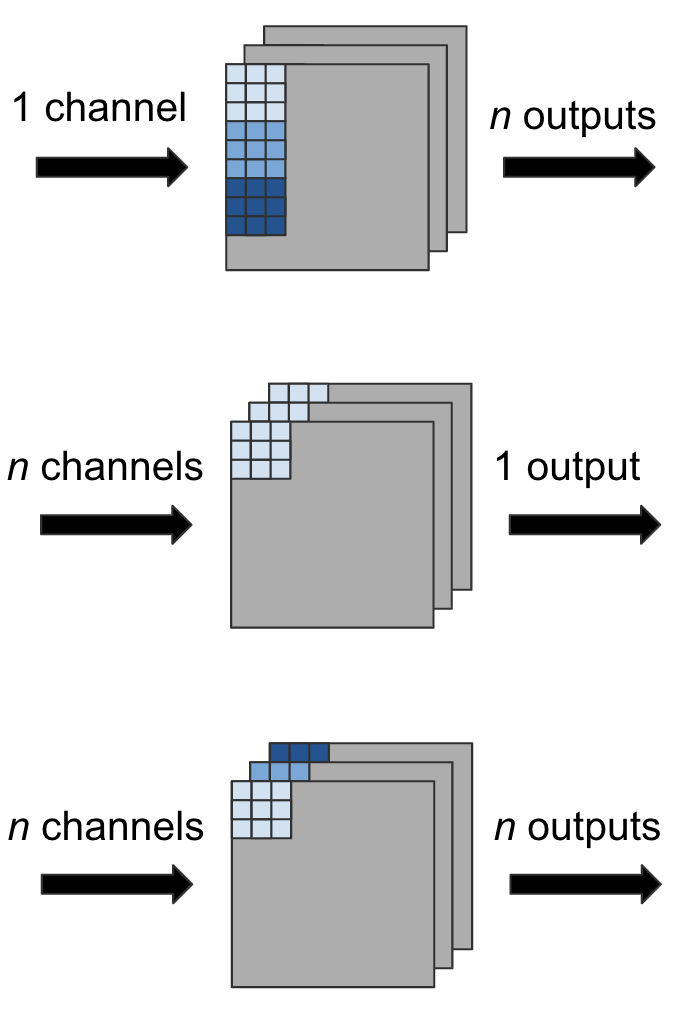
\includegraphics[scale=0.45]{ccu_parallelism}
	\caption[CCU Channel-Wise Parallelism]%
	{\narrower Channel-wise convolution oriented to either reuse inputs, outputs, or stay independent.}
	\label{ccuparallelism}
\end{wrapfigure}

Our CCU component computes a single channel's worth of convolution. \ref{ccuparallelism} shows how channel-wise parallelism can be oriented to either reuse inputs, outputs, or be entirely independent. In the case of reusing inputs, a mechanism must be in place to insure atomic updates are made to the output layer to prevent concurrent CCUs from overwriting values. In conjunction with one of these orientations, channel computation can be iterated to reuse existing input channels for different kernels altogether, continue on the kernel's next channel to complete the current output layer, or reuse the same kernel on a different input within a mini-batch. Input and kernel sizes could drastically impact memory latencies for each orientation. Our work focuses primarily on the acceleration of a single reconfigurable CCU. Thus, we leave the exploration of CCU parallelism slated for future work.

The logic of our reconfigurable CCU component is depicted in \ref{convolver}. Note that subsequent diagrams do not have a one-to-one correspondence with their actual hardware implementation due to the HLS translation. We use a sliding window mechanism similar to \cite{liu2016automatic} with the exception that ours is reconfigurable for any sized input, with a fixed kernel size of three. We choose three because its one of the more popular kernel sizes (REF NEEDED). We can compute convolution for different sized kernels using a technique similar to \cite{guo2018angel} where they pad outer weights with zero for smaller kernels and perform multiple convolutions using subsets and zero-padding for larger kernels.

We first load three rows from external RAM into the input data buffer, implemented in on-chip RAM. Its size is set to fit three of the largest input layer's rows, which consequently wastes BRAM resources when computing smaller layers. A sliding 3x3 window then strides along the rows, loading the current values within the window into registers to multiply and accumulate them with the kernel weights into the output buffer. Once the three rows are complete, we transfer the output buffer data to external RAM.


\begin{figure}
	\centering
	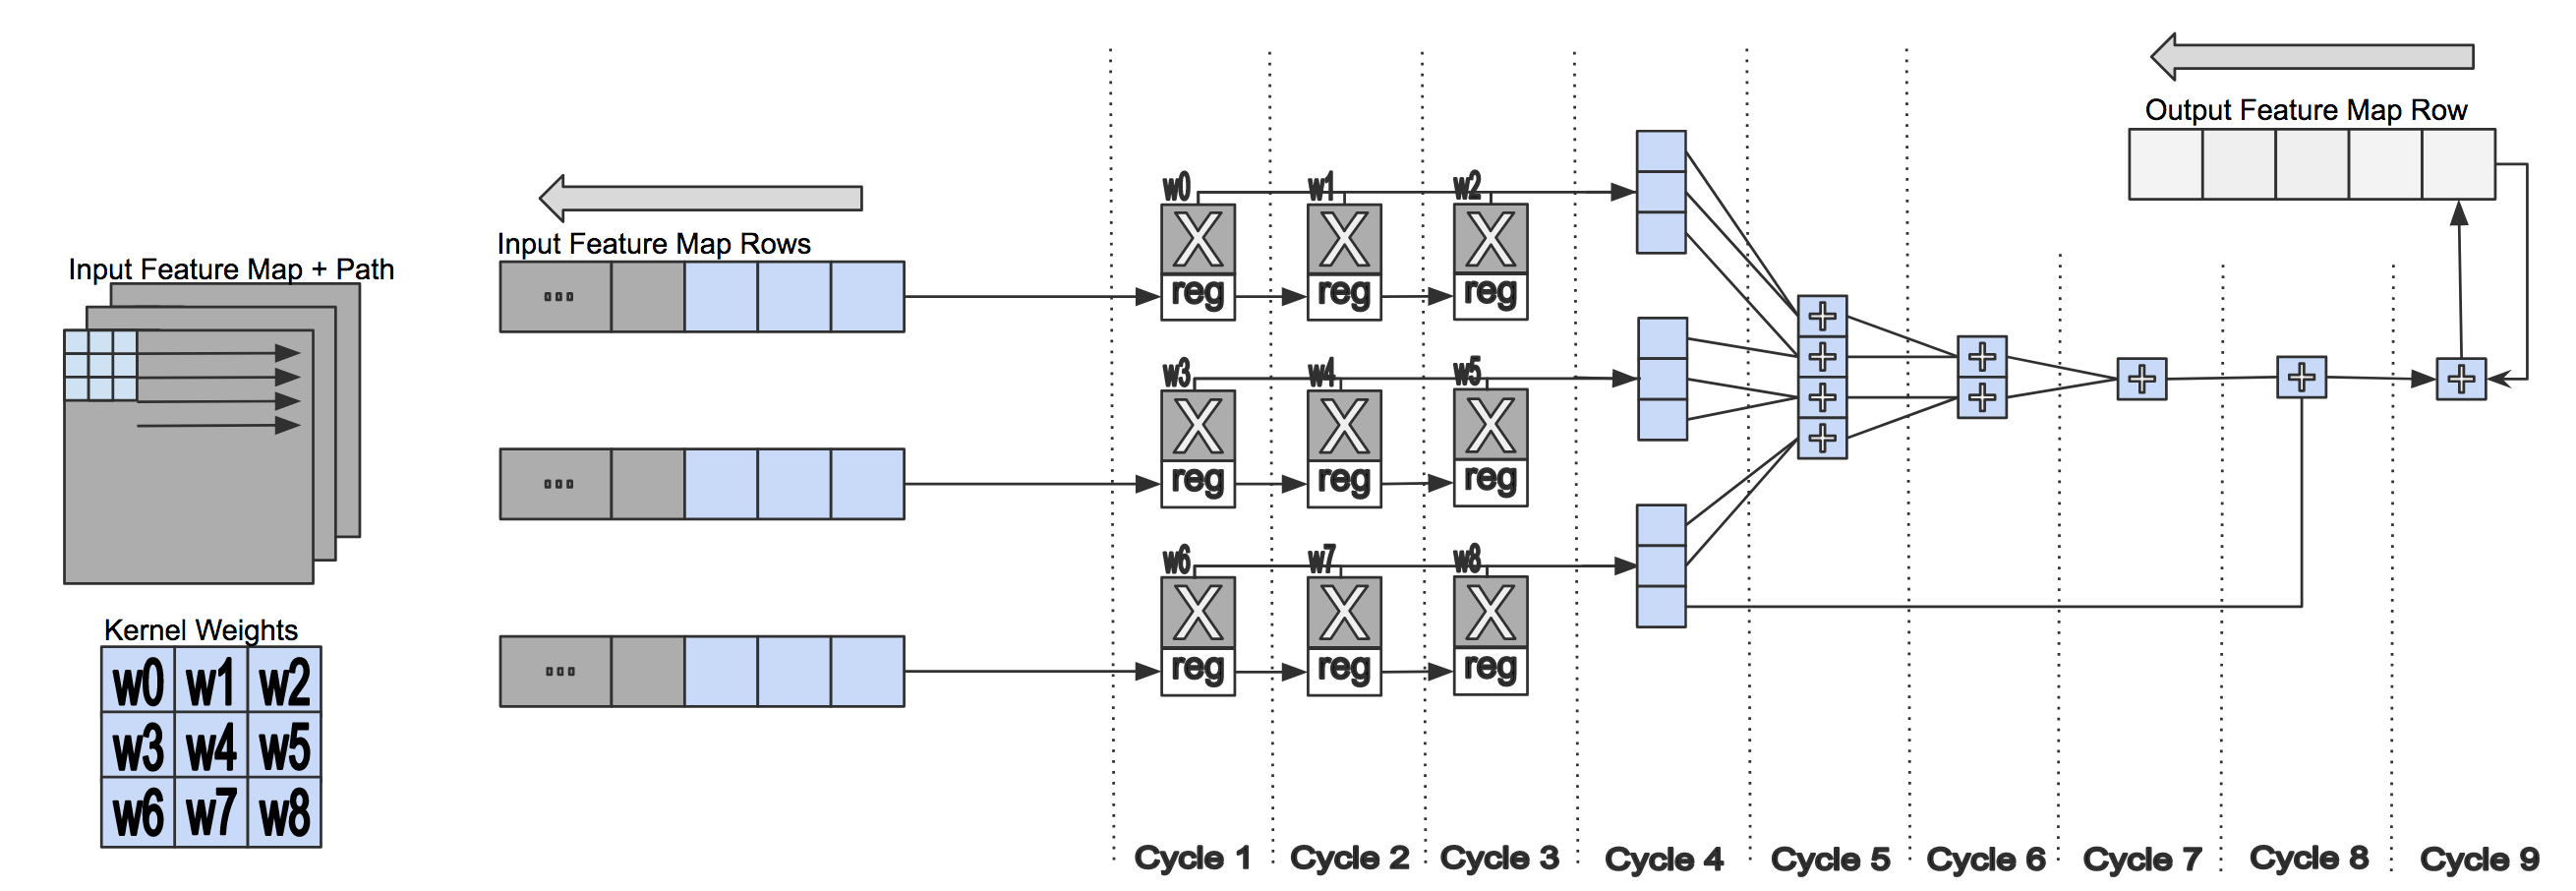
\includegraphics[scale=0.35]{ConvolverDiagram}
	\caption[Convolver Diagram]%
	{\narrower Sliding window CCU with a 3x3 kernel. Loads three rows into RAM and performs a sliding window to load values into registers and compute the convolution.}
	\label{convolver}
\end{figure}


\section{Environment and Experimental Results}
We implement our reconfigurable CCU using the Intel HLS Compiler specifically for the Cyclone V. Benchmarks and correctness tests are obtained and verified using the ModelSim FPGA simulator. Each benchmark is ran using artificial data with input dimensionality, padding, and kernel sizes set to respective layer sizes from the VGG-16 architecture. Floating point quantization is set to 16 bit precision throughout all benchmarks. For OPs, we consider only multiplies and accumulates and take into account the padding. We compute GOP/s by fixing the clock speed to 100 MHz.

Results show our CCU's performance scales near-consistent for input sizes greater than 28. Smaller input sizes pay the penalty of refilling the input data buffer more frequently, shortening the phase of pipelined convolution. 


\begin{figure}
\centering
\begin{tabular}{ |p{3cm}|p{3cm}|p{3cm}|p{3cm}|  }
	\hline
	\multicolumn{4}{|c|}{3x3 Convolution, Single Channel, Padding=1, Stride=1, 100 MHz} \\
	\hline
	Size & Cycles & OPs & GOP/s \\
	\hline
	7x7       & 1433      & 882      & 0.062\\
	14x14    & 3938     & 3528    & 0.09 \\
	28x28   & 10174    & 14112    & 0.139\\
	56x56   & 42568   & 56448  & 0.133\\
	112x112  & 172815  & 225792 & 0.131 \\
	224x224 & 812774  & 903168 & 0.111\\
	
	\hline
\end{tabular}
\label{result_1}
\caption{Benchmarks of our sliding window CCU}
\end{figure}


% ADD PART REGARDING MODEL SIM FPGA PARAMS LIKE MAKE, ETC

